\chapter{Teoretický základ}
\label{2-teorie}

Tato kapitola si klade za cíl seznámit čtenáře s~teoretickými základy měření radioaktivity, z~nichž
plyne potřeba posunu. Dále pak načrtne způsoby, kterými bude možno body posouvat, a~popíše
nejdůležitější problémy, s~nimiž se při takovém posunu lze setkat. 

\section{Scintilační spektrometrie}
\label{spektrometrie}

Ježto lidský subjekt není sám o~sobě schopen detekovat ionizující záření, je třeba si vypomoci příslušnou
technikou, tedy přístroji, detektory ionizujícího záření. Tako\-vých přístrojů existuje velké
a neustále se zvětšující množství. 

Obecně se detektory dělí buď podle průběhu detekce v závislosti na čase (kumulativní a~kontinuální),
nebo podle principu detekce (materiálové, fotografické a~pro nás nejdůležitější elektronické). 

  \begin{figure}[H]
   \centering
	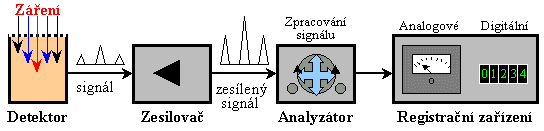
\includegraphics{./pictures/elektronicky-detektor.png}
	\caption[Základní schéma elektronického detektoru záření]{Základní schéma elektronického
	detektoru záření
	(zdroj: \cite{spektrometrie})}
      \label{fig:elektronicky-detektor}
  \end{figure}

Běžný elektronický detektor ionizujícího záření se skládá ze dvou hlavních bloků - z~detektorové
a~analyzační části. V~detektoru dochází k~transformaci ionizačního záření na měřitelné
elektronické impulsy. Takové impulsy bývají zesilovány buď už v~detektoru, nebo v~následujícím
zesilovači; často se užívá kombinace obého. Signál zesílený na měřitelnou odezvu poté putuje do
analyzátoru, který uživateli předává informace buď analogovou formou (například výchylka ručičky),
nebo formou di\-gitální (číselný ukazatel, zápis do souboru v~počítači). 

Následující podkapitoly představí přístroj a~metodu současně velice využívané,
totiž scintilační spektrometry. Scintilační spektrometry patří do elektronických detektorů
a~pro naši práci je důležité, že se objevují též v terénním měření \zk{SÚRO}. 

  \begin{figure}[H]
   \centering
	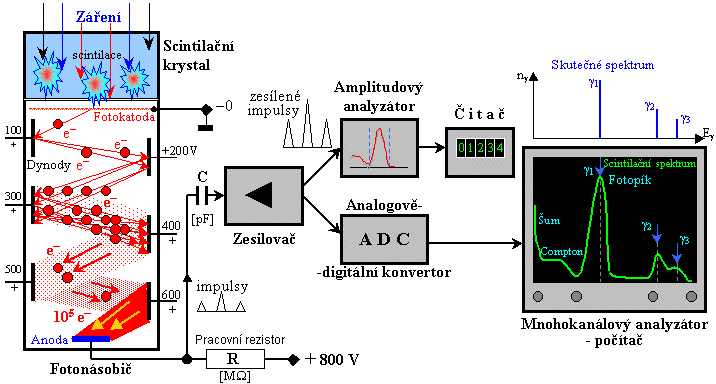
\includegraphics[scale=0.75]{./pictures/scintilacni-detektor.png}
	\caption[Obecné schéma scintilačního detektoru]{Obecné schéma scintilačního detektoru
	(zdroj: \cite{spektrometrie})}
      \label{fig:scintilacni-detektor}
  \end{figure}

\subsection{Detektorová část}
\label{detektor}

Ve scintilačních detektorech zachycuje ionizační záření takzvaná scintilační sonda.
Ta sestává ze scintilačního krystalu a~fotonásobiče umístěných ve světlotěsném pou\-zdře.
Pouzdro nejen že zabraňuje vniku nadbytečného světla do detekční jednotky, ale také stíní
vnější magnetické pole, které by mohlo ovlivňovat správnou funkci fotonásobiče. 

Obecná práce scintilačního detektoru spočívá v~tom, že detekuje-li nějaké ionizační záření, dochází ve
scintilačním krystalu ke světelným zábleskům. Emise fotonů jsou přímo úměrné absorbovanému záření.
Pomocí fotoelektrického jevu je ve vstup\-ní fotokatodě fotonásobiče převedeno fotonové kvantum na kvantum
elektronové, načež uvnitř fotonásobiče dojde k zněkolikanásobení elektronů. 

\subsubsection{Scintilační krystal}
\label{krystal}

Existují látky, takzvané scintilátory, které na pohlcení kvant ionizujícího záření reagují
scintilacemi (z~latinského scintilla~-~jiskra\footnote{zdroj: FÜRST, Kamil a MEISSNER, Josef:
\textit{Slovník latinsko-český a česko-latinský}, Praha: Nakladatelé Kvasnička a Hampl, 1941}, scintilace
tedy představují světel\-né záblesky).
Byť se mohou objevovat i~scintilátory kapalné či plynné, zde se budeme zabývat scintilátory
nejběžněji užívanými - krystaly. 

Krystaly bývají planárního válcového tvaru, případně pro speciálnější účely (vy\-soko\-energetická záření,
detekce měkkého záření gama) velkoobjemové, studnové či tenké. V~současné době jsou krystaly
nejčastěji vyráběny z~jodidu sodného aktivovaného thaliem (\textit{NaI(Tl)}), dříve se též
používal sirník zinečnatý aktivovaný stříbrem nebo kyanid platino-barnatý. 

Pokud bychom scintilátor jen přivařili ke vstupnímu okénku fotonásobiče, dochá\-zelo by
ve vzduchové vrstvě mezi výstupním okén\-kem scintilátoru a vstupním okén\-kem fotonásobiče k~nechtěné
ztrátě fotonů. Tento prostor tedy bývá zaplňován látkou s~vysokou světelnou vodivostí, například
silikonovou vazelínou. V~případě většího průzvu bývají oba elementy spojeny světlovodičem či
optickými vlákny. 

\subsubsection{Fotonásobič}
\label{fotonasobic}

Fotonásobič představuje optoelektronickou součástku, která na základě fotoelektrického jevu
převádí světelný tok na elektrické signály. Jeho výhoda tkví ve vysoké citlivosti způsobené
několikanásobným zvětšením počtu elektronů pomocí dynod, pročež lze i~z~jediného fotonu
vyprodukovat dobře detekovatelný elektronický impuls. Fotonásobič tak navzdory svému názvu nenásobí
fotony, nýbrž elektrony vyvolané prvotním dopadem fotonů na fotokatodu. 

Vstupním elementem fotonásobiče je tedy fotokatoda. Jedná se o~tenkou vrstvu napařenou na
vstupním okénku, tvořenou zejména antimonidy alkalických prvků (nejčastěji cesia a antimonu),
ana převádí dopadající fotony fotoelektrickým jevem na elektrony.
Tenkost tvoří důležitou součást její výroby; v~opačném případě by mohlo docházet k~pohlcování
emitovaných elektronů v~materiálu fotokatody. 

Za fotokatodou (mezi fotokatodou a~první dynodou) se může nacházet kladně nabitá mřížka.
Její kladné napětí udává emitovaným elektronům vyšší rychlost a~usměrňuje je na první z~dynod. 

Následně tyto vyloučené elektrony násobí sekundární emise na dynodách. Dy\-nody představují soustavu
zvláštních elektrod, kde se na každou následující přivádí vyšší (zpravidla o~100~V nebo
dvojnásobné) kladné napětí, pročež přitahují emitované elektrony. Tento systém funguje
jako elektronový zesilovač. Každá z~dynod pracuje tím způsobem, že po nárazu jednoho elektronu emituje
další elektrony. Mezi počtem vyražených elektronů a~kinetickou energií dopadajícího elektronu
platí přímá úměra. Obvykle se počet elektronů na každé dynodě zdvojnásobí. Několikerým
mrdáním elektronů dojde k~jejich množení geometrickou řadou. Dynody mívají zpravidla
zakřivený tvar (vhodnější pro fokusaci elektronů na další dynodu). 

Posledním prvkem pak jest anoda - sběrná elektroda s~nejvyšším napětím, z~níž už přes pracovní
odpor \textit{R} pokračuje výstupní signál do zesilovače, případně přímo do analyzační části. 

  \begin{figure}[H]
   \centering
	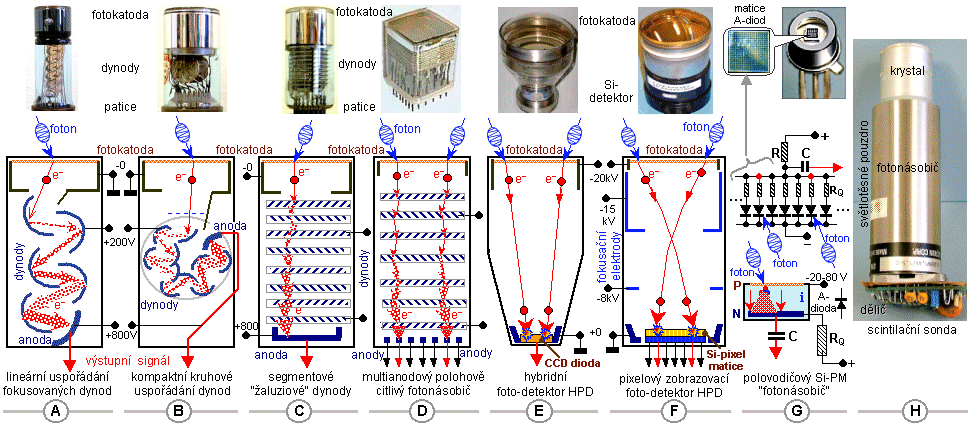
\includegraphics[scale=0.5]{./pictures/fotonasobice.png}
	\caption[Různá uspořádání fotonásobičů]{Různá uspořádání fotonásobičů
	(zdroj: \cite{spektrometrie})}
      \label{fig:fotonasobice}
  \end{figure}

\subsection{Analyzační část}
\label{analyzator}

Zesílené elektrické signály je třeba dále analyzovat. Existují dva druhy analyzátorů,
které prezentují v~obrázku \ref{fig:scintilacni-detektor} dvě paralelní větve. 

V~případě amplitudového analyzátoru se měří počet impulsů s~amplitudou mezi nastavenými
diskriminačními hladinami. Diskriminační hodnoty představují amplitudové infimum a~supremum.
Amplitudy ležící mimo toto rozmezí nebudou k~čítači propuštěny. Tím se částečně
eliminují chyby a~temný proud - proud protékající fotonásobičem i~bez ozáření fotokatody.
Územ bývá nastavit toto rozmezí tak, aby obsahovalo fotopík (pík totální absorpce) záření
měřeného radionuklidu. Impulsy zkrácené o~přebytečné hodnoty následně vstoupí již do čítače impulsů. 

Spektrometrická analýza vyžaduje transformaci impulsů na bitové informace; k~té dochází
v~analogově-digitálním převodníku. V~paměti počítače se každé amplitudě záření gama
střádacím algoritmem přidělí buňka. Při detekci takového kvanta se její hodnota zvyšuje o~1.
Takovým postupem získáme scintilační spektrum, jehož grafické
znázornění je na obrázku \ref{fig:scintilacni-detektor}. 

\section{Sběr souřadnic a potřeba posunu}
\label{potreba posunu}

Sběr měření probíhá letecky. Scintilační spektrometr je uložen ve vrtulníku, který přelétá nad zkoumaným
územím; při přeletu se v~spektrometru registrují hodnoty záření. Tato data jsou registrována v~podstatě
neustále, ale zapisují se až po jistém časovém úseku (běžně po vteřině) jako průměr hodnot za onen
časový úsek měřených. V~okamžiku zápisu hodnot radionuklidů se rovněž tak zapisují zeměpisné souřadnice
(a~další parametry). Ty se však nijak neprůměrují, zapisují se momentální hodnoty. 

Z~popsaného plyne, že se registrované zeměpisné souřadnice od souřadnic geometrického průměru snímaného
pole liší; jedná se o~souřadnice začátku nebo konce měření v~dané epoše (záleží na použitém přístroji).
Vzniká tedy potřeba korekce zpoždění/předbíhání záznamu souřadnic oproti měřeným hodnotám. 

\section{Posun}
\label{posun}

Bohužel není k~dispozici záznam výšek vrtulníku během letu, ani přesný záznam jeho rychlosti, tudíž
není možnost dokonalé souřadnicové korekce, různými algoritmy se ale ideální hodnotě můžeme alespoň
přiblížit. Zásuvný modul umožňuje tři základní posuny měřených dat. 

Nejjednodušším způsobem je posun o~hodnoty. Hodnotě každého bodu přiřadíme souřadnice bodu
předcházejícího či následujícího (s~libovolným krokem). Takový posun ovšem nijak neposouvá jednotlivé
body, alebrž jen vzájemně vyměňuje jejich souřadnice. Před vývojem zásuvného modulu byl však tento
\textit{posun} tím zdaleka nejvyužívanějším, téměř bezkonkurenčně, pro svou jednoduchost - stačilo
posunout sloupce s potřebnými daty o~zamýšlený počet hodnot. 

  \begin{figure}[H]
   \centering
	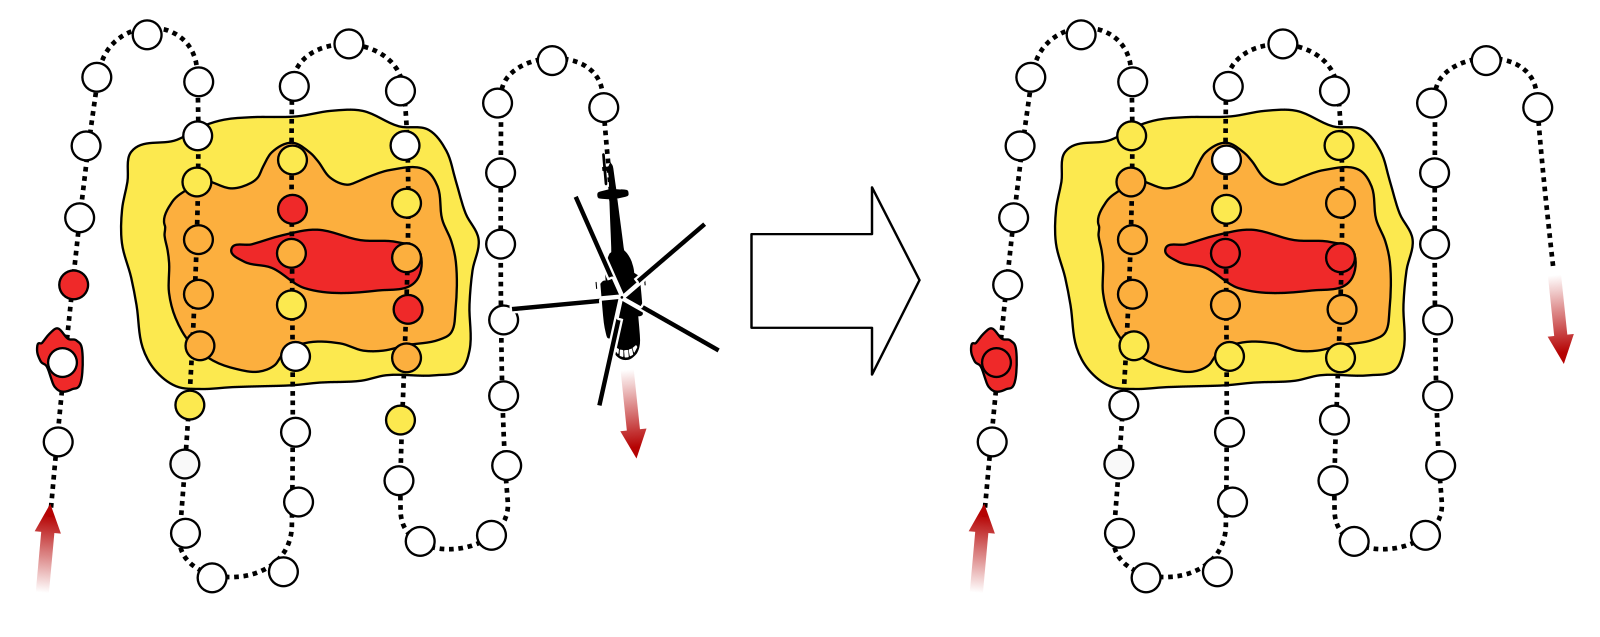
\includegraphics[scale=0.2]{./pictures/posun.png}
	\caption[Posun dat o 1 hodnotu]{Posun dat o 1 hodnotu
	
	(zdroj: HELEBRANT, Jan a GRYC, Lubomír: \textit{GPS position lag correction} [interní dokument
	SÚRO, v.v.i.])}
      \label{fig:posun}
  \end{figure}

Nápaditěji působí posun o~konstantní vzdálenost. Uživatel dostane možnost posunout všechny body
po trajektorii letu o~jím volenou vzdálenost. Tento princip představuje již skutečný, realitu lépe
vystihující posun. V~ideálním případě popsaném na následujících obrázcích by posun o~14 metrů přesunul
body na jejich náležité místo. 

  \begin{figure}[H]
   \centering
	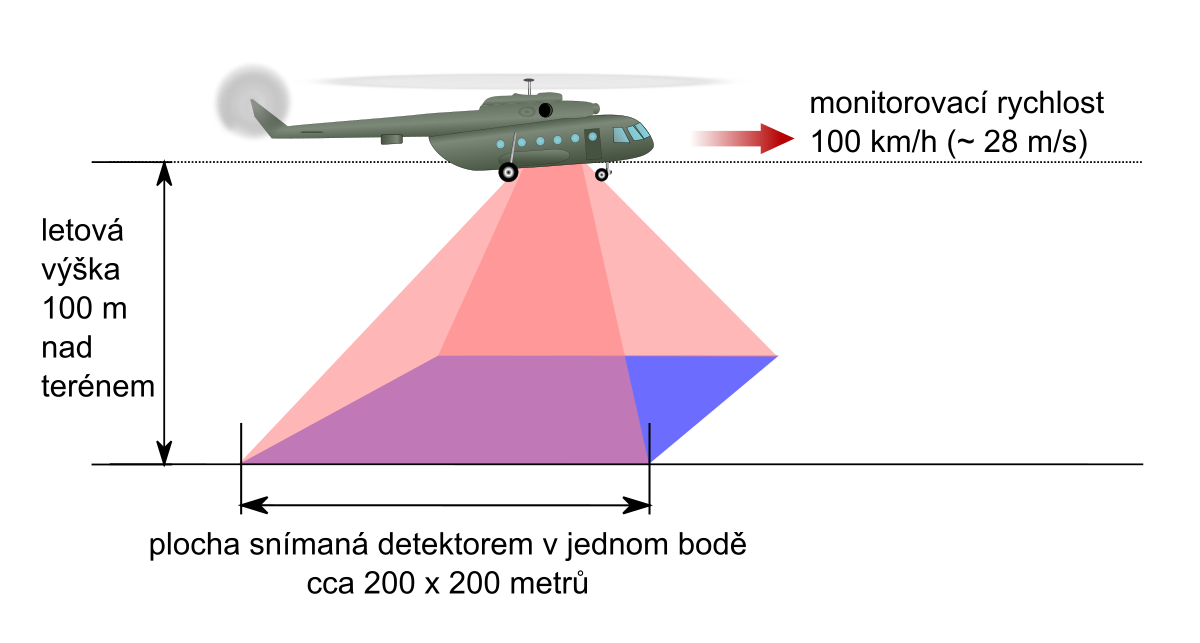
\includegraphics[scale=0.4]{./pictures/snimani.png}
	\caption[Princip měření]{Princip měření
	
	(zdroj: HELEBRANT, Jan a GRYC, Lubomír: \textit{GPS position lag correction} [interní dokument
	SÚRO, v.v.i.])}
      \label{fig:mereni}
  \end{figure}
  
  \begin{figure}[H]
   \centering
	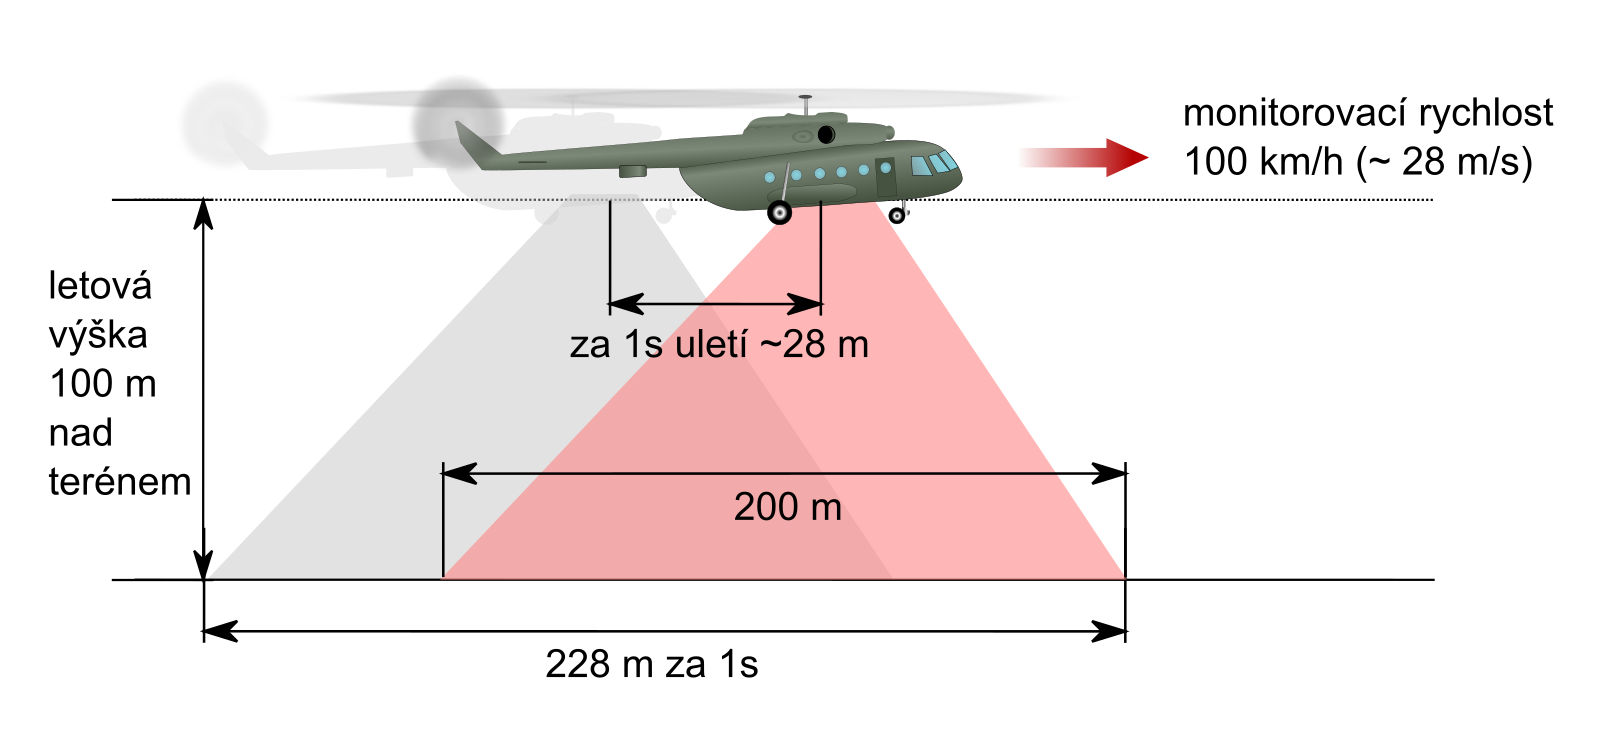
\includegraphics[scale=0.3]{./pictures/snimani-detail.png}
	\caption[Profilové schéma měření]{Profilové schéma měření
	
	(zdroj: HELEBRANT, Jan a GRYC, Lubomír: \textit{GPS position lag correction} [interní dokument
	SÚRO, v.v.i.])}
      \label{fig:mereni-profil}
  \end{figure}
  
Skutečnosti nejvěrněji odpovídá posun o~sekundy. V~dřeni se jedná o~posun o~vzdálenost, ale tentokráte
nikoli konstantní. 

Ze známých zeměpisných souřadnic se mezi každou dvojicí bodů vypočte vzdále\-nost. Neboť známe pro každý
z~bodů časovou značku, lehce (rozdíl dvou hodnot) vypočteme dobu, za niž vrtulník tuto vzdálenost urazil.
Tím získáme veškeré potřebné veličiny pro výpočet rychlosti mezi dvěma body. Následuje postup opačný:
Na zá\-kladě uživatelem zadané doby, o~niž se mají body posunout, se vypočte vzdálenost, kterou by
vrtulník za danou dobu urazil. Vztáhneme-li tuto vzdálenost opět na trajektorii pohybu, obdržíme
souřadnice posunutého bodu. 

\section{Problémy}
\label{problemy}

Při tvorbě zásuvného modulu, který by jmenované operace umožňoval, může dojít k~mnoha nepříjemnostem
a~mnoha problémům, s~nimiž je třeba se vypořádat. Jmenujme alespoň dva nejdůležitější: 

\subsection{Elipsoid}
\label{elipsoid}

Ačkoli různé typy spektrometrů produkují odlišné výstupy a~některé mohou obsahovat i~zeměpisné souřadnice
na jiném referenčním tělese, zpravidla obsahují (také) souřadnice na elipsoidu \zk{WGS84}. 

Přítomnost elipsoidických souřadnic namísto rovinných vnáší do výpočtu záludnou diafragmu, na niž musí
tvůrce algoritmu dbát zvýšeného zřetele. Od výpočtů na referenční kouli (nerci v~rovině) se
zásadně liší nejen délka, ale také azimut. Nejkratší spojnice (takzvaná geodetická křivka) pak samozřejmě
nepředstavuje v~rovinném zobrazení úsečku. Majoritu těchto problémů vyřešíme užitím první základní
geodetické úlohy na elipsoidu. 

\subsection{První geodetická úloha}
\label{prvnigu}

První geodetická úloha představuje hledání (výpočet) parametrů bodu na konci křivky, v~případě
představovaného zásuvného modulu na referenčním elipsoid. Zná\-mými parametry jsou souřadnice počátečního
bodu křivky a~její azimut v~tomto bodě. Hledanými parametry zeměpisné souřadnice koncového bodu.
Zkoumaná křivka reprezentuje geodetickou křivku. 

Základní geodetické úlohy se dají řešit nejedním způsobem a~v~minulosti vždy znamenaly mnohé potíže
a~dlouhé výpočty. S~rozvojem informačních technologií došlo k~značnému urychlení výpočtu.
Prezentovaný princip vychází z~principu popisovaného v~\cite{vyssigeodezie} a~vycházejícího
z~postupu Ing.~Jana Douši. 

Postup spočívá v~rozdělení křivky na integrační kroky. Křivku, resp.~její úsek~\textit{h}
aproximujeme polynomem čtvrtého stupně, takzvanou Runge-Kuttovou metodou řádu~4. Potíž spočívá v~tom,
na kolik úseků máme danou křivku rozdělit. Přesnost totiž ovlivňuje nejen délka křivky, ale také její
poloha na elipsoidu. 

Daný problém řeší postupné iterace. Křivka se postupně půlí, následně se půlí její poloviny atd. (jde
tedy o~\textit{1/n}~násobky původní délky, kde \textit{n} představuje mocniny dvou), než dosáhneme
požadované přesnosti. Ta je kontrolována pomocí podmínky cyklu: Pokud se od sebe všechny vypočtené
atributy koncového bodu křivky ve dvou po sobě jdoucích iteracích liší o~hodnotu menší než danou
(v našem případě 0.0000000001~úhlového stupně), jsou poslední vypočtené atributy brány jako výsledné. 


  \begin{figure}[H]
   \centering
	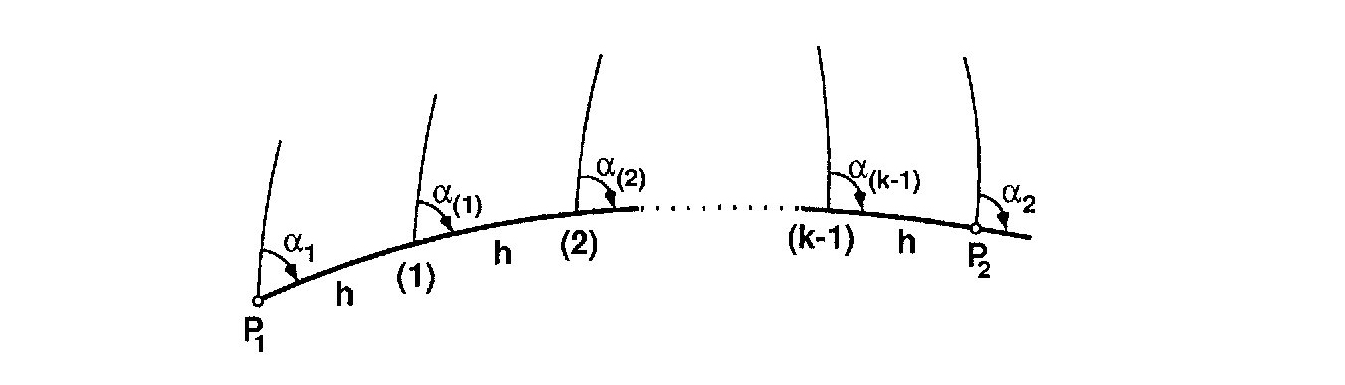
\includegraphics[scale=0.4]{./pictures/prvnigu-integrace.png}
	\caption[Integrační kroky v první geodetické úloze]{Integrační kroky v první geodetické úloze
	(zdroj: \cite{vyssigeodezie})}
      \label{fig:prvnigu-integrace}
  \end{figure}





